\documentclass[conference]{IEEEtran}
\IEEEoverridecommandlockouts
% The preceding line is only needed to identify funding in the first footnote. If that is unneeded, please comment it out.
\usepackage{cite}
\usepackage{amsmath,amssymb,amsfonts}
\usepackage{algorithmic,array}
\usepackage[ruled,noline,linesnumbered,noend]{algorithm2e}
\usepackage{graphicx}
\usepackage{textcomp}
\usepackage{xcolor}

% algorithm styling
\SetInd{0.5em}{0.2em}       % reduce indent
\newcommand\mycommentfont[1]{\footnotesize\sffamily{#1}}
\SetCommentSty{mycommentfont}

% fun with colors
\RequirePackage{color}
\usepackage{colortbl}
\definecolor{RED}{rgb}{1,0,0}
\definecolor{BLUE}{rgb}{0,0,1}
\definecolor{GREEN}{rgb}{0,1,0}
\definecolor{color1}{rgb}{0.913, 0.776, 0.686}
\definecolor{color2}{rgb}{0.913, 0.867, 0.686}
\definecolor{ltgray}{rgb}{0.85, 0.85, 0.85}

% notes, remarks, todo
\newcommand{\Remark}[1]{{\color{RED}\sf Remark: {#1}}}
\newcommand{\tp}[1]{{\color{RED}\sf TP: {#1}}}
\newcommand{\dm}[1]{{\color{BLUE}\sf DM: {#1}}}
\newcommand{\Fix}[1]            {\textcolor{red}{\small\sf [#1]}}
\newcommand{\kw}[1]             {{\tt #1}\xspace}
\newcommand{\todo}[1]{
      \addcontentsline{tdo}{todo}{\protect{#1}}
      \marginpar{\colorbox{white!90!black}{\textcolor{red}{
      \parbox{2.1cm}{\scriptsize\bf\raggedright #1}
      }}}
}

\newcommand{\eqt}[1]{Equation.~(\ref{#1})}
\newcommand{\fig}[1]{Fig.~(\ref{#1})}
\newcommand{\sect}[1]{Section.~(\ref{#1})}
\newcommand{\algo}[1]{Algorithm.~(\ref{#1})}

\usepackage{etoolbox}

\usepackage{wrapfig}
\usepackage{pgfplots}
\usepackage{tikz}
\usetikzlibrary{arrows}
\usetikzlibrary{decorations.shapes}
%\pgfplotsset{width=10cm,compat=1.9}
\usetikzlibrary{arrows.meta}
\usetikzlibrary{calc}

\tikzset{
	myarrow/.style={-{Triangle[length=3mm,width=1mm]}}
}

\usepackage[norndcorners,customcolors,nofill]{hf-tikz}
\hfsetbordercolor{black!50}


\def\BibTeX{{\rm B\kern-.05em{\sc i\kern-.025em b}\kern-.08em
    T\kern-.1667em\lower.7ex\hbox{E}\kern-.125emX}}
\begin{document}

\title{Parallel Domain Decomposition Techniques Applied to Multi-Variate Functional Approximation of Discrete Data\\
%{\footnotesize \textsuperscript{*}Note: Sub-titles are not captured in Xplore and should not be used}
%\thanks{Identify applicable funding agency here. If none, delete this.}
\thanks{Early Career Research Program, Department of Energy, US}
}

\author{\IEEEauthorblockN{1\textsuperscript{st} Vijay S. Mahadevan}
\IEEEauthorblockA{\textit{Mathematics and Computational Science Division} \\
\textit{Argonne National Laboratory}\\
Lemont, IL, 60439, USA \\
mahadevan@anl.gov}
\and
\IEEEauthorblockN{2\textsuperscript{nd} Thomas Peterka}
\IEEEauthorblockA{\textit{Mathematics and Computational Science Division} \\
\textit{Argonne National Laboratory}\\
Lemont, IL, 60439, USA \\
tpeterka@mcs.anl.gov}
\and
\IEEEauthorblockN{3\textsuperscript{rd} Iulian Grindeanu}
\IEEEauthorblockA{\textit{Mathematics and Computational Science Division} \\
\textit{Argonne National Laboratory}\\
Lemont, IL, 60439, USA \\
iulian@anl.gov}
\and
\IEEEauthorblockN{4\textsuperscript{th} Youssef Nashed}
\IEEEauthorblockA{\textit{Stats Perform}\\
Chicago, IL, 60601, USA \\
youssef.nashed@statsperform.com}
}

\maketitle

\begin{abstract}
Compactly expressing large-scale datasets through multivariate functional approximations (MFA) can be critically important for analysis and visualization to drive scientific discovery. This paper presents a data and domain partitioning approach to scalably compute a MFA representation, by reducing the total work per task in combination with a nonlinear Schwarz-type, inner-outer iterative scheme for converging the interface data. For the underlying MFA, we utilize a tensorial expansion of non-uniform B-spline (NURBS) basis to adaptively reduce the functional approximation error in the input data. While previous work on adaptive NURBS-based MFA has been proven successful, the computational complexity for encoding large datasets on a single process can be prohibitive. We demonstrate effectiveness of the presented approach with an overlapping Jacobi additive Schwarz method (JASM) based domain decomposition solver, with a nonlinear accelerator such as L-BFGS or Krylov (CGS, L-GMRes) to minimize the subdomain error residuals obtained from decoding the MFA, and more specifically to resolve the discontinuities at boundaries. The analysis of the presented scheme for some analytical and real scientific datasets in 1-D and 2-D are also presented. Additionally, scalability studies are also shown for some real-world 2-d datasets to evaluate the parallel speedup of the algorithm on large clusters.
\end{abstract}

\begin{IEEEkeywords}
functional approximation, domain decomposition, scalable methods
\end{IEEEkeywords}

\section{Introduction}

Large scale discrete data analysis from various scientific computational simulations often require high-order continuous functional representations that have to be evaluated anywhere in the domain. Such expansions described as Multivariate Functional Approximations (MFA) in arbitrary dimensions \cite{nurbs-book} allow the original discrete data to be compressed, and expressed in a compact closed form in addition to supporting higher-order derivative queries. One particular option is to use NURBS bases for the MFA encoding of scattered data \cite{peterka-mfa}. Due to the potentially large datasets that need to be encoded into a MFA, the need for computationally efficient algorithms (in both time and memory) to partition the work into subtasks is critically important. 

In the current paper, we utilize domain decomposition (DD) techniques \cite{smith-ddm} with data partitioning strategies to produce scalable algorithms to adaptively compute the MFA to reproduce a given dataset within user-specified tolerances. In such partitions, it is imperative to ensure that the continuity of the data across subdomain interfaces are maintained and is consistent with the degree of the underlying bases used in the MFA. 
We present an iterative DD scheme with an outer Schwarz-type iterative scheme in order to ensure that continuity is recovered, and the overall error stays bounded when number of subdomains are increased (subdomain size decreases).

%{\color{red}THIS IS A DRAFT}

%\begin{itemize}
%	\item Talk about MFA and how it can be used to approximation discrete solution data. Reference previous work.
%	\item Provide motivations on why this is necessary especially for large datasets
%	\item Literature survey of other work for parallel interpolation and compression of data
%	\item What are the other approaches to address this issue; pros and cons
%\end{itemize}

The paper is organized as follows. Section 2 summarizes the related work in using variations of the Schwarz scheme for scalably interpolating data, and using constraints for recovering continuity along discontinuous patches. Section 3 provides details about the constrained optimization problem to resolve subdomain boundary discontinuities, along with the outer-inner DD based solver setup to compute the continuous MFA. Next the application of the DD solver for 1-D/2-D analytical problems are provided to verify error convergence, and scalability of the hierarchical scheme with decreasing subdomain size under overlap specifications. Finally, the parallel scalability of the scheme is presented for some real-world cases to adaptively compute the MFA within user-specified tolerances.


\section{Related Work}

DD techniques for parallel interpolation of scattered data has been explored previously with Radial Basis Functions (RBF) \cite{mai-approx-rbf}, yielding good scalability to create a MFA that closely replicates underlying profile. Overlapping variants of multiplicative and additive Schwarz iterative techniques for RBF \cite{ddm-rbf} have been proven successful to tackle large problems. Additionally, use of restricted Additive-Schwarz preconditioners with Krylov iterative solvers have been shown to be scalable \cite{yokota-rasm-rbf} for such problems as well. However, using NURBS-basis to compute MFA in parallel, while maintaining higher-order continuity across subdomains has not been explored previously in this context. To overcome the issues with discontinuities along NURBS patches, \cite{zhang-nurbs-continuity} have proposed to use a gradient projection scheme to constrain the value ($G_0$), the gradient ($G_1$) and the hessian ($G_2$) at a small number of test points for optimal shape recovery. 

Application of NURBS basis to high-fidelity modeling of nonlinear PDEs have also enjoyed recent success \cite{petiga-dalcin-2016} at scale, but the current implementations lack full support for handling multiple patches in a distributed memory setting.  Alternatively, it is possible to create a constrained recovery during the actual post-processing stage i.e., during the decoding stage of the MFA through blending techniques \cite{grindeanu-blending}, in order to recover continuity in the decoded data. However, the underlying MFA representation would still remain discontinuous, and would become more so with increasing number of subdomains. In contrast, we propose an extension to the constrained solvers used by \cite{zhang-nurbs-continuity, xu-jahn-discrete-adjoint} by utilizing a recursive DD-based parallel outer-inner iterative scheme to resolve continuity prescriptions as required by the user. The outer iteration utilizes a flavor of the restricted Additive-Schwarz method (RASM) \cite{gander-rasm}, with an efficient, inner subdomain solver using L-BFGS as used in \cite{zheng-bo-bspline-bfgs}, or Krylov-type schemes (CGS, L-GMRes) to minimize the decoded residual within acceptable error tolerances. This DD solver has low memory requirements that scales with growing subdomains, and only imposes nearest neighbor communication of the interface data once per outer iteration. 

\section{Approach}

Domain decomposition techniques in general rely on the idea of splitting a larger domain into smaller subdomains, which results in coupled Degrees-of-Freedom (DoF) at their common interface. Typical applications in Boundary-Value problems (BVP) \cite{smith-ddm, lions-asm} have been employed successfully for efficiently computing the solution to large Partial Differential Equations (PDEs) with DD in a scalable fashion. In the current work, we utilize a data decomposition approach, with possibility of overlapping or shared layers such that higher-order continuity across domain boundaries are preserved in order to generate consistent and accurate MFA representations in parallel. Similar to overlapping Schwarz solvers for PDE applications, the amount of overlap in the data for MFA directly affects the convergence speed and scalability of the overall algorithm. And the overall accuracy of the parallel algorithm cannot be worse than the single subdomain case.

For illustration, consider a 1-D domain ($\Omega$) with two partitions (number of subdomains $n_s=2$) as shown in \fig{fig:DD-subdomain-illiustration}, where $\Omega_1$ and $\Omega_2$ represent the subdomains that share an interface $d\Omega_{1,2}$. If the scheme is invoked with an overlap layer $\Delta$, the corresponding overlaps are also shown as $\Delta_1$ and $\Delta_2$.

\tikzset{decorate sep/.style 2 args=
	{decorate,decoration={shape backgrounds,shape=circle,shape size=#1,shape sep=#2}}}

\begin{figure}
\centering
\begin{tikzpicture}
\begin{scope}[very thick]
\begin{axis}[cycle list name=exotic, legend style={draw=none}, axis lines=none, xtick=\empty, ytick=\empty, xmin=0, xmax=100, ymin=0.8, ymax=1.2]
%\begin{axis}[legend style={draw=none},xmin=-5, xmax=105, ymin=0.8, ymax=1.2]

\addplot[domain=0:50, samples=6, color=blue, mark=halfcircle] {1.0};

\addplot[domain=50:100, samples=6, color=red, mark=halfcircle] {1.0};
%\addplot[color=blue] coordinates {0,0.5} ;
%\addplot +[mark=none] coordinates {(0.5,1.25) (0.5,0.75)};
%\addplot[domain=0.5:1, samples=6, color=black] {1};
%\addplot coordinates {(0,1) (0.1,1) (0.2,1) (0.3,1) (0.4,1) (0.5,1) (0.6,1) (0.7,1) (0.8,1) (0.9,1) (1,1)};
%\draw[decorate sep={1mm}{2mm},fill] (0,0) -- (100,0);
%\draw[myarrow] (0,0) -- (1,5.5);

\draw [decorate,decoration={brace,mirror,amplitude=20pt},color=blue,xshift=0pt,yshift=70pt]
(0,0.9) -- (50,0.9) node [black,midway,yshift=-1cm] 
{\footnotesize $\Omega_1$};

\draw [decorate,decoration={brace,mirror,amplitude=5pt},color=blue,xshift=0pt,yshift=70pt]
(50,0.9) -- (60,0.9) node [black,midway,yshift=-5mm] 
{\footnotesize $\Delta_1$};

\draw [decorate,decoration={brace,amplitude=20pt},color=red,xshift=0pt,yshift=90pt]
(50,1.1) -- (100,1.1) node [black,midway,yshift=1cm] 
{\footnotesize $\Omega_2$};

\draw [decorate,decoration={brace,amplitude=5pt},color=red,xshift=0pt,yshift=90pt]
(40,2.1) -- (50,2.1) node [black,midway,yshift=5mm] 
{\footnotesize $\Delta_2$};

\addplot [dashed, black, thick] coordinates {(50,1.15)  (50,0.85)} node[above left] {\footnotesize $\Omega_{1,2}$ } ;

\end{axis}
\end{scope}
\end{tikzpicture}
\caption{1-D Parallel Partitioned Domain}
\label{fig:DD-subdomain-illiustration}
\end{figure}


It is imperative to note that the only exchange of data between subdomains is performed through nearest neighbor communication that has bounded complexity and costs. The volume of messages exchanged however depends on several factors.
\begin{enumerate}
	\item \textbf{Continuity}: The degree of continuity determines the stencil needed to enforce the constraints on either side of the interface
	\item \textbf{Overlap}: The number of overlap layers in the data determines the control point data coupling to be communicated between neighboring domains
\end{enumerate}


%\begin{itemize}
%	\item What are we proposing and why this can be a stable technique to recover high-order continuity in parallel ?
%	\item Give context about DD methods and how ASM in this context makes sense 
%	\item Refer to \cite{smith-ddm} and \cite{ddm-rbf} as well and write out the equations with \cite{nurbs-book} help
%\end{itemize}

\subsection{Solver Methodology}
\label{sec:solver-methodology}

A pth degree NURBS curve \cite{nurbs-book} is defined using the Cox-deBoor functions as

\begin{eqnarray}
C(u) &=& \sum_{i=0}^{n} R_{i,p}(u) P_i, \forall u \in \Omega \\
R_{i,p}(u) &=& \frac{N_{i,p}(u) w_i}{\sum_{i=0}^{n} N_{i,p}(u) w_i}
\label{eq:nurbs-basis}
\end{eqnarray}

where $R_{i,p}(u)$ are the piecewise rational functions with $P_i$ control points, $w_i$ weights and p-th degree B-spline basis $N_{i,p}(u)$ defined on a knot-vector $U$. Exact high-order derivatives of these NURBS basis defined in \eqt{eq:nurbs-basis} can also be evaluated without any approximation errors at the control point locations.

Given a set of input points that need to be encoded $Q$, the linear Least-Squares (LLS) fitting algorithm can be applied to compute the control point data. This results in a normal form of linear equations to be solved as follows.

\begin{equation}
(N_i^T R_i) P_i = N_i^T Q_i, \forall i \in [1, \ldots n_s]
\label{eq:LSQ-system}
\end{equation}

The iterative scheme used in the current work utilizes the unconstrained LLS solve as the first initial guess $P_{LS}$ to compute the optimal solution in each subdomain. Once $P_{LS}$ is available for the individual subdomains, the global nonlinear problem with subdomain boundary constraints can be written out as
%
\begin{equation}
A(X) X = F, \quad X = \left[P1 ; P2 \right]
\label{eq:global-system}
\end{equation}

where
\begin{eqnarray}
A(X) &=&
\left[
\begin{array}{c|c}
A_{1,1}(P_1) & A_{1,2}(P_1,P_2) \\
\hline
A_{2,1}(P_1,P_2) & A_{2,2}(P_1)
\end{array}
\right], \\ 
&\quad& \nonumber \\
F &=& \left[
\begin{array}{c}
N_1^T Q_{1} \\
N_2^T Q_{2}
\end{array}
\right]
\label{eq:coupled-operator}
\end{eqnarray}

The diagonal operators $A_{1,1}$ and $A_{2,2}$ correspond to the linear operator that minimizes the local subdomain residuals while the off-diagonal blocks $A_{1,2}$ and $A_{2,1}$ represent the coupling terms between the subdomains at $\Omega_{1,2}$. This coupling term contains the constraints on the shared control points, its derivatives and the weights along subdomain boundaries, satisfying which will enforce solution continuity in the global MFA representation. 

The coupling blocks can also be reformulated to introduce Lagrange multipliers to explicitly couple the control points, derivatives and weights across a subdomain interface such that continuity is preserved in a weak sense \cite{nurbs-book}. In the current paper, we instead use the Schur complement of \eqt{eq:coupled-operator} to eliminate the coupling terms by evaluating it at the lagged iterate values, in order to impose constraints in each subdomain independently. Hence, the coupled data $P_2, W_2$ and $P_1, W_1$ for subdomains $\Omega_1$ and $\Omega_2$ respectively are exchanged simultaneously before the local domain solves are computed. Since the exchanged constraint data is lagged, it can slightly slow down iteration convergence in comparison to the more expensive multiplicative Schwarz variants \cite{smith-ddm}. The key advantage of this block-Jacobi type operator leading to the restricted additive Schwarz method (RASM) is that it only requires nearest neighbor exchange of data, that keeps communication costs bounded as number of subdomains increase \cite{gander-rasm}. Note that in a Jacobi-Schwarz outer iterative scheme, nearest neighbor exchanges can be performed compactly per dimension and direction, thereby minimizing communication costs and eliminating global collectives.

Once the interface constraint data terms are received, a Schur complement of \eqt{eq:coupled-operator} can be computed to eliminate the coupling terms, and to impose constraints in each subdomain independently. This leads to an augmented subdomain solution as shown in \eqt{eq:augmented-solution} that includes the control point, and optionally the derivative and weights at the interface obtained from the adjacent subdomain. 

\begin{equation}
%\tikzset{left offset=-0.1,right offset=0.02,disable rounded corners=true}
\tikzset{offset def/.style={
		above left offset={-0.1,0.8},
		below right offset={0.1,-0.65},
	}
}
%\begin{array}{@{} *{2}{ c @{} >{{}}c<{{}} @{} } c @{}}
%16\cdot \tikzmarkin{A}I_1  & + & 11\cdot \tikzmarkin{B}I_2  & = & \tikzmarkin{C}13\\[1ex]
%11\cdot I_1\tikzmarkend{A} & + & 16\cdot I_2\tikzmarkend{B} & = & 17\tikzmarkend{C}
%\end{array}
P_1^{'} =
\left[
\begin{array}{c}
\tikzmarkin{A}(1,-0.3)(-0.1,0.3) P_1(1)   \\
P_1 (2) \\
\vdots   \\
\tikzmarkend{A} P_1 (m) \\
$\quad$ \vspace*{-2mm} \\
\tikzmarkin{B}(0.6,-0.1)(-0.1,0.3) P_2(1) \\
0 \\
\vdots \\
\tikzmarkend{B} 0
\end{array}
\right],
P_2^{'} =
\left[
\begin{array}{c}
\tikzmarkin{C}(1,-0.3)(-0.1,0.3) P_2(1)   \\
P_2 (2) \\
\vdots   \\
\tikzmarkend{C} P_2 (n) \\
$\quad$ \vspace*{-2mm} \\
\tikzmarkin{D}(0.6,-0.1)(-0.1,0.3) P_1(1) \\
0 \\
\vdots \\
\tikzmarkend{D} 0
\end{array}
\right]
\label{eq:augmented-solution}
\end{equation}
%
\begin{tikzpicture}[remember picture,overlay]
\pgfsetarrowsend{latex} 
%
% adjust the shift from "col" to move the position of the annotation
\coordinate (A-aa) at ($(A)+(-0.5,-1.0)$);
\node[align=left,left] at (A-aa) {\footnotesize{$P_1$($\Omega_1$)}};
\path[>=stealth,blue,draw] (A-aa) -- ($(A)+(0.2,-1.0)$);
%
% adjust the shift from "col" to move the position of the annotation
\coordinate (B-aa) at ($(B)+(-0.5,-1.0)$);
\node[align=left,left] at (B-aa) {\footnotesize{$P_1$($\Delta_1$)}};
\path[>=stealth,blue,draw] (B-aa) -- ($(B)+(0.2,-1.0)$);
%
% adjust the shift from "col" to move the position of the annotation
\coordinate (C-aa) at ($(C)+(1.4,-1.0)$);
\node[align=right,right] at (C-aa) {\footnotesize{$P_2$($\Omega_2$)}};
\path[>=stealth,red,draw] (C-aa) -- ($(C)+(0.75,-1.0)$);
%
% adjust the shift from "col" to move the position of the annotation
\coordinate (D-aa) at ($(D)+(1.4,-1.0)$);
\node[align=right,right] at (D-aa) {\footnotesize{$P_2$($\Delta_2$)}};
\path[>=stealth,red,draw] (D-aa) -- ($(D)+(0.75,-1.0)$);
%
\end{tikzpicture}
%
where $m, n$ are the number of control points in $\Omega_1$ and $\Omega_2$ respectively.

At convergence, the interface data at $\Omega_{1,2}$ will satisfy the continuity prescriptions specified by the user ($G_0$, $G_1$, $G_2$). The illustration and description can be generalized and extended to arbitrary dimensions and will be used as the basis for the local subdomain solvers introduced further in the following subsections.

\subsection{Constrained Linear Least-Squares Solver}

Given the user specification to obtain a $G_0, G_1$ or $G_2$ continuity across block interfaces, the local subdomain solve can essentially be formulated as the solution to a LSQ problem with constraints. The idea here is to introduce additional unknowns in the solutions, which are essentially the Lagrange multipliers to obtain an augmented system of equations.

If we consider the local system introduced in \eqt{eq:LSQ-system}, the solution $P$ is the unconstrained control point data that is only piecewise continuous globally. Then, we can introduce a constrained set of equations \cite{nurbs-book} such that 

\begin{equation}
(N_i^T M_i) P_i = N_i^T T_i, \forall i \in [1, \ldots n_s]
\label{eq:LSQ-system-constraint}
\end{equation}

where $M$ is the basis matrix corresponding to the constrained DoFs and $T$ is the vector of input data in the overlap region of interest $\Delta$. Then the constrained linear least squares curve fitting problem is simply minimizing the residual $E=Q-RP$ such that $MP=T$ is satisfied. We refer the readers to Section (9.4.2) in \cite{nurbs-book} for further details on how a Schur complement of the coupled equation systems can be applied to eliminate the Lagrange multipliers in order to enforce the constraints within each subdomain system. This particular strategy can also be extended to higher dimensions easily with larger number of constraints included in the $M$ operator.

\subsection{Constrained Nonlinear Solver}

In order to ensure continuity across NURBS patches, Zhang et al  \cite{zhang-nurbs-continuity} evaluated the constraint matrix at test points along the interface curve. These computations require a Singular Value Decomposition (SVD) solve at every interface and can become prohibitively expensive as dimensionality increases. Alternatively, we can use a nonlinear minimizer, directly applied to the system in \eqt{eq:LSQ-system}, and adding a penalized term for the constrained DoFs. Such a system can be expressed as a scalar minimization problem in each subdomain with the following objective functional.
%
\begin{eqnarray}
%r_1 &=& (Q_1 - R_1 P_1) + \epsilon \left[ (P_1(\Delta_1) - P_2(\Omega_2 \cap \Delta_1 )) \right], \forall P_1 \in \Omega_1  \\
%%
%r_2 &=& (Q_2 - R_2 P_2) + \epsilon \left[ (P_2(\Delta_2) - P_1(\Omega_1 \cap \Delta_2)) \right], \forall P_2 \in \Omega_2 
r_i(\Omega_i) &=& Q_i - R_i P_i \nonumber \\
r_c(\Delta_{i})    &=& \sum_{\partial \Omega_i} \left[ \delta_{i,\partial \Omega} (P_i(\Delta_i) - P_{i+1}(\Omega_{i+1} \cap \Delta_{i} ))  \right]^2 \nonumber \\ 
r_i(\Omega_i \bigcup \Delta_{i}) &=& \left\lVert r_i(\Omega_i) \right\rVert_2 + \epsilon r_c(\Delta_{i}), \forall i \in [1, n_s]
%&+& \epsilon \left[ (1-\delta_{i,0}) (P_i(\Delta_i) - P_{i+1}(\Omega_{i+1} \cap \Delta_{i} ))  \right]^2 \nonumber \\ 
%&+& \epsilon \left[ (1-\delta_{i,n_s}) (P_i(\Delta_{i}) - P_{i-1}(\Omega_{i-1} \cap \Delta_i)) \right]^2, \nonumber \\
%r_i^2 &=& \left\lVert Q_i - R_i P_i \right\rVert_2 \nonumber \\
%&+& \epsilon \left[ (1-\delta_{i,0}) (P_i(\Delta_i) - P_{i+1}(\Omega_{i+1} \cap \Delta_{i} ))  \right]^2 \nonumber \\ 
%&+& \epsilon \left[ (1-\delta_{i,n_s}) (P_i(\Delta_{i}) - P_{i-1}(\Omega_{i-1} \cap \Delta_i)) \right]^2, \nonumber 
\label{eq:nonlinear-residuals}
\end{eqnarray}

where $\epsilon$ is the boundary penalty term, typically set to $10^{7}$ and $\delta_{i,j}$ is the Kronecker delta.

The augmented solution for each local subdomain after nearest neighbor exchange can contain control points and corresponding derivative data to constrain DoFs on both the left and right interfaces in 1-D. This definition can be extended naturally to higher dimensions, and hence the penalized constraints on the boundary terms can be evaluated as a loop over all shared interfaces to compute the net residual. The minimizer in terms of the control point solution is achieved when the interface solutions match on either side to drive the nonlinear residuals to zero.

To compute the 	solution to the minimization problem, we can make use of Sequential Least SQuares Programming (SLSQP) solver with equality constraints, or apply the limited memory version of  Broyden-Fletcher-Goldfarb-Shannon algorithm (BFGS), L-BFGS algorithm, when then dimension size increases, and memory requirements become large. Such solvers have already been proven effective for converging such constrained continuity problems with B-Splines \cite{zheng-bo-bspline-bfgs}. A more efficient method is to reformulate the objective function in \eqt{eq:nonlinear-residuals} in to a root finding problem, by expressing it as a residual vector to be minimized for all components. Then Krylov accelerators or Anderson mixing can be applied to compute the optimally constrained solutions to such problems with much lower computational complexity due to faster convergence properties of the scheme.

%A much more efficient solver would also be to use a Krylov accelerator for the subdomain solves, which expresses the components in \eqt{eq:nonlinear-residuals} as a vector to reformulate it as a root finding problem. In our experiments, the Krylov accelerator was typically much faster to converge and compute the optimally constrained solutions.

\subsection{Constrained Nonlinear Solver on Decoded Data}

Instead of imposing the constraints in the control point space, alternatively, we can utilize the expansion of the MFA in input point space directly to minimize the decoded residual $E= Q - R P$. There are some advantages to this approach compared to imposing the interface constraints in the control point space, even though the potential volume of data to be communicated between subdomains is much larger.

\begin{enumerate}
	\item Subdomain residuals and boundary constraints are both in the decoded space, and hence no explicit need for a residual projection (encoding) or penalty term in \eqt{eq:nonlinear-residuals}
	\item No explicit need for imposition of higher order derivative constraints, especially in the context of non-conforming adaptivity across subdomain interfaces
	\item Natural extensions within the ASM iterative scheme to generate overlapping variants
\end{enumerate}

%Explain the iterative scheme in terms of the underlying equations and how the boundary terms are resolved through a global ASM method. First start with 1-d and talk about extensions in the scheme to allow arbitrary dimensional solver framework.

When the solver is setup to use the error residuals in the actual decoded space, the natural data decomposition with overlap $\Delta$ can yield good improvements in both time and accuracy. This follows the effectiveness of the overlapping additive-Schwarz preconditioning schemes in the context of linear algebra problems for PDEs \cite{smith-ddm} \cite{gander-rasm}. 

%\begin{equation}
%(N_i^T M_i) P_i = N_i^T T_i, \forall i \in [1, \ldots n_s]
%\label{eq:decoded-residuals}
%\end{equation}


\subsection{Implementation}
\label{sec:implementation}

The presented methods in this manuscript have been primarily implemented in Python using interfaces to the DIY C++ library. DIY~\cite{morozov16} is a programming model and runtime
for block-parallel analytics on distributed-memory machines, built on MPI-3~\cite{dongarra13}.  Rather than programming
for process parallelism directly in MPI, the programming model in DIY is based on block parallelism: data are decomposed
into subdomains called blocks; blocks are assigned to processing elements (processes or threads); computation is
described over these blocks, and communication between blocks is defined by reusable patterns. The same DIY program
consisting of a block-parallel decomposition can be run on different numbers of MPI processes: it is the job of the DIY
runtime to map between blocks and processes. The Python bindings to DIY, pyDIY~\cite{pydiy},
are a more recent development that utilize PyBind11~\cite{jakob17} and MPI4Py~\cite{dalcin11} to expose the interfaces in the C++ library. Note that in the current implementation, PyDIY and DIY exclusively manage the data decomposition, including specifications to share an interface $\Omega_{i,j}$ and ghost layers that represent overlaps $\Delta$.

The overall approach is sketched in \algo{alg:pseudocode}.
% \Remark{Vijay: finish the pseudocode and expand the discussion of it below.} 
We begin by decomposing the domain into a set of regular blocks aligned with the principal axes
of the global domain. Before enforcing constraints, the local subdomain solves are performed completely decoupled so that the discontinuous MFA to represent the partitioned input data is computed. We then begin iterating over the blocks in a 2-level nested loop: the outer loop is driven by RASM
iterations described in \sect{sec:solver-methodology}, while the inner loop executes the individual subdomain MFA solves simultaneously to compute the control point solution to the nonlinear optimization problem in \eqt{eq:LSQ-system-constraint} or \eqt{eq:nonlinear-residuals}
% -- \ref{eq:decoded-residuals} 
with BFGS or Krylov methods. 
At the start of each outer ASM iteration, the control point constraints are exchanged between neighboring blocks in a regular nearest-neighbor communication pattern. This is sufficient to update the constraints $P(\Delta)$ for the inner subdomain solves. The DIY send and receive data exchange API is responsible to enqueue and dequeue the constraint data based on the data decomposition.
While there are many different subdomain solver methodologies presented before, the current implementation ensures that the net residual for the local block is converged adaptively with knot placements to capture solution data and gradient variations.
At the end of the outer iterative loop, we check for convergence across all subdomains, by evaluating whether the maxima of the $L_{\infty}$ error across all subdomains ($n_s$) of the ASM update vector is within user-specified tolerance. If this condition is satisfied, the MFA computation is stopped.
On convergence, the hierarchic iterative procedure computes the global MFA that retains higher order continuity and accuracy of a single subdomain solve, but with excellent parallel efficiency to reduce total time to solution with growing subdomains.


\Remark{\algo{alg:pseudocode} is just a skeleton. Details need to be filled in. Termination conditions, local
(inner loop) iterative scheme, types of constraints (control points or decoded points), etc.}

\begin{algorithm}
    \DontPrintSemicolon
    decompose domain into blocks with DIY\;
    solve local MFA without constraints\;
    \tcp*[h]{Outer ASM loop;}\;
    iASM $\leftarrow$ 0\;
    \While{ dPMax $ > 10^{-10}$ and iASM $<$ nMaxASM}
    {
        $P(\Omega \cap \Delta)$ $\rightarrow$ enqueue outgoing constraints\;
        exchange constraints with neighbor blocks\;
        $P(\Delta)$ $\leftarrow$ dequeue incoming constraints\;
        \tcp*[h]{Inner BFGS/Krylov optimization loop}\;
        \For {$isub \in n_s$}
        {
            $P_i \leftarrow$ solve adaptive local MFA with constraints\;
            $E_i \leftarrow$ compute decoded local error\;
            $\delta P (\Omega_i) \leftarrow P_{iASM} (\Omega_i) - P_{iASM-1} (\Omega_i)$\;
        }
        dPMax $\leftarrow \left\lVert \delta P (\Omega_i) \right\rVert_{\infty}$\;
    	iASM++\;
    }
    \caption{\Remark{Hierarchic DD MFA Solver}}
    \label{alg:pseudocode}
\end{algorithm}



\section{Results}
\label{sec:results}

To demonstrate the effectiveness of the nested iterative algorithm, we utilize both analytical closed form functionals and scientific datasets in both 1-D and 2-D obtained from high-fidelity simulations. A brief description of the problem cases that are used as test datasets are given below.

\begin{enumerate}
	\item Synthetic data: sinc($x$)=$\frac{sin(x)}{x}$ functional on $\Omega \in [-4, 4]$
	\begin{itemize}
		\item 1-D: Q = (sinc($x$) + sinc(2*$x$-1) + sinc(3*$x$+1.5)), 
		\item 2-D: Q = (sinc($\sqrt{x^2+y^2}$))
	\end{itemize}
	\item Nek5000: A 3-D dataset from CFD simulation with velocity magnitude as the solution profile
	\item S3D: This is a 3-D turbulent combustion dataset generated by an S3D simulation \cite{chen-s3d-2009} of fuel jet combustion in the presence of an external cross-flow. 
	\item CESM: A 2-D Community Atmosphere Model climate model dataset on a sphere with 3600x1800 resolution
\end{enumerate}


\subsection{1-D Results}\label{AA}

%\begin{itemize}
%	\item Use the first two problems to measure convergence in parallel as number of domains increase
%	\item Talk about adaptivity and resolution of data even for highly varying problem data.
%\end{itemize}

\subsubsection{Adaptive Error Convergence and Verification}

The 1-D implementation of the ASM iterative solver was applied to the sinc problem. An initial input problem size of 500 points was evaluated as a test case, and MFA representation for the resulting profile was computed on 4 subdomains. The solution profile, along with the control point locations from the adaptive computation are shown in \fig{fig:sinc-adaptive-a}. We utilized the residual definition shown in \eqt{eq:nonlinear-residuals} with a $G_1$ constraint to be satisfied along all internal subdomain interfaces. The \fig{fig:sinc-adaptive-b} and \fig{fig:sinc-adaptive-c} present the zoomed in reconstruction of the approximation near the interface between $\Omega_2$ and $\Omega_3$ before, and after the ASM iterations are converged. The discontinuous representation of data when performing independent, adaptive, unconstrained subdomain solves are converged to satisfy the constraints after only 3 RAS iterations, with nearest neighbor exchange of control point data at the interfaces to recover $G_1$ continuity.

\begin{figure}
	\centering
	\subfloat[sinc function profile in 1-D\label{fig:sinc-adaptive-a}]{%
		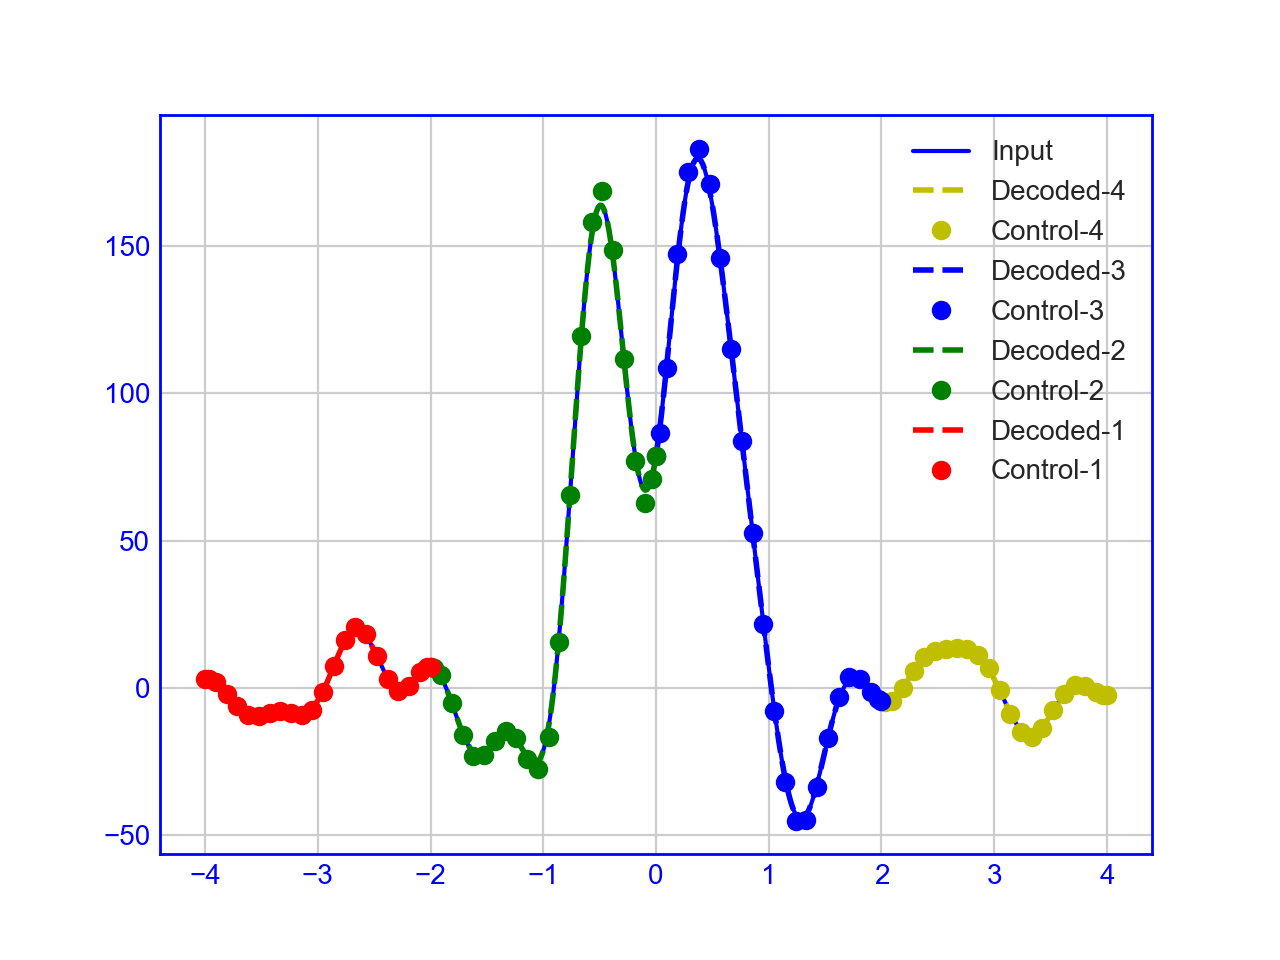
\includegraphics[width=0.5\textwidth]{figures/sinc-1d-profile}}
	\hfill
	\subfloat[Zoomed in image of $\Omega_{2,3}$ at (a) iASM=0\label{fig:sinc-adaptive-b}]{%
		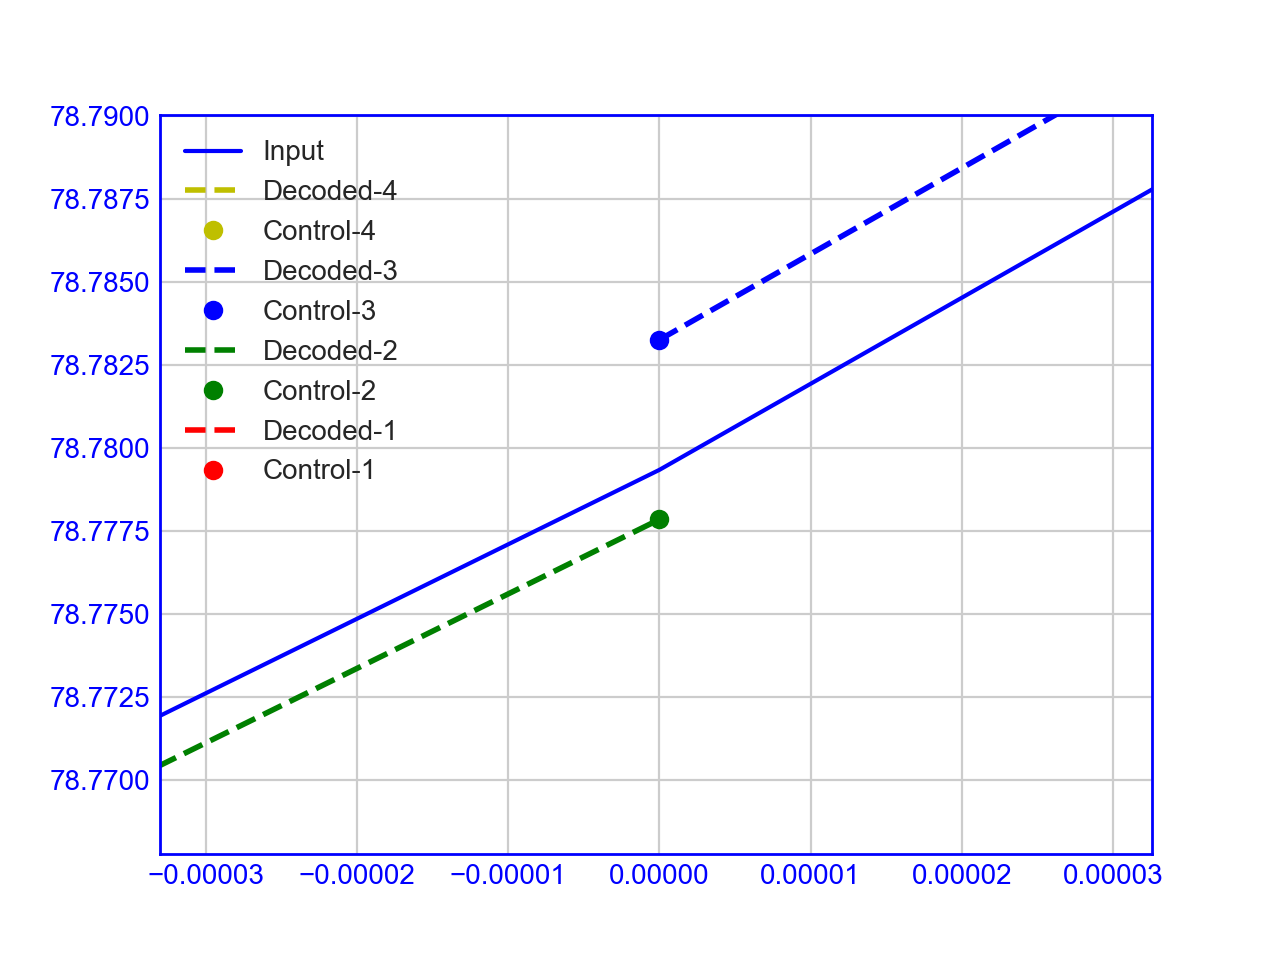
\includegraphics[width=0.5\textwidth]{figures/sinc-1d-discontinuous}}
	\\
	\subfloat[Zoomed in images of $\Omega_{2,3}$ at iASM=3\label{fig:sinc-adaptive-c}]{%
		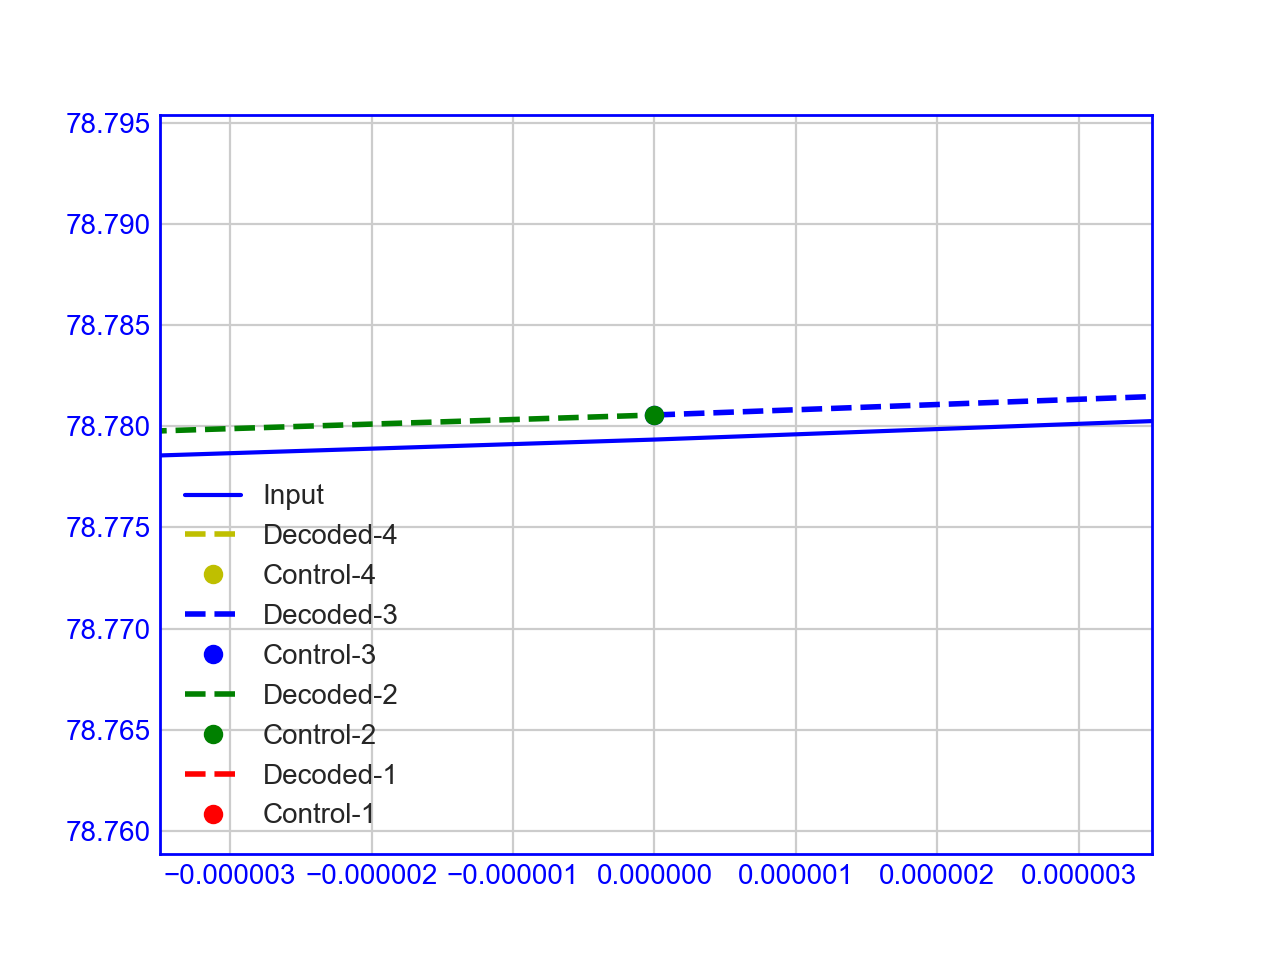
\includegraphics[width=0.5\textwidth]{figures/sinc-1d-continuous}}
	\caption{1-D analytical sinc dataset with 501 input points: adaptive MFA on 4 subdomains with $10^{-4}$ 	tolerance and $p=2$}
	\label{fig:sinc-adaptive}
\end{figure}

%\subsubsection{Subdomain Solver Performance}
%
%Compare LCLSQ - Encoded nonlinear and Decoded nonlinear

\subsubsection{Overlap Experiments in 1-D}

In this 1-D experiment on the closed form sinc function shown in \sect{sec:results}, we utilize the decoded residual minimization with the ASM-Krylov solver combination, and increase the amount of overlap in the input points to look at convergence speed. We measured the global $L_2$ error convergence along with the total cost in terms of outer iteration to compute the constrained control point locations. In this analysis, adaptivity in the individual subdomains was explicitly turned off so as to maintain a constant ratio of input points to control points per subdomain, as overlap region is extended in the subdomains on both the left and right sides.

\fig{fig:decoded-overlap-data-performance} shows the global $L_2$ norm of the net error in the decoded residual, as the number of subdomains are increased. With no overlap regions, where only the interface data is shared, the total ASM iterations needed to satisfy convergence, and the net error increase monotonically with $n_s$. As the overlap size becomes larger, for $\Delta=32$ and $\Delta=64$, the error growth and the iterations required remain much more bounded in comparison to the non-overlapping case. The implications of this particular result closely matches the DD ASM preconditioning theory often applied in PDE solvers \cite{smith-ddm, lions-asm, gander-rasm}. It also shows that the RAS iterative scheme can be accelerated more efficiently, and scalably used as a solver without a prohibitive linear complexity of O($n_s$).

\begin{figure}
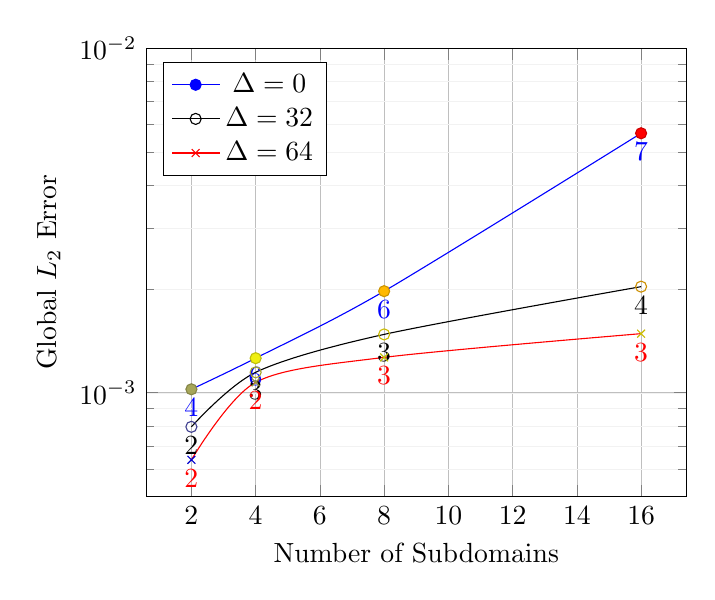
\begin{tikzpicture}

\begin{semilogyaxis}[
legend pos= north west,
ymin = 0.0005, ymax = 0.01,
xlabel=Number of Subdomains,
ylabel=Global $L_2$ Error,
nodes near coords*={\Label},
visualization depends on={value \thisrow{label} \as \Label},
grid=both,
grid style={line width=.1pt, draw=gray!10},
major grid style={line width=.2pt,draw=gray!50},
axis line style={latex-latex},
%axis lines=middle,
]
\axispath\draw
(7.49165,-10.02171)
|-  (8.31801,-11.32467)
node[near start,left] {$\frac{dy}{dx} = -2.58$};

\addplot[smooth,mark=*,blue] table [meta=class]  {
	x y class label
	2    0.001023481 A 4
	4    0.001259901 B 6
	8    0.001971792 C 6
	16   0.005663382 D 7
};

\addplot[smooth,mark=o,black] table [meta=class]  {
	x y class label
	2    0.000796565 A 2
	4    0.001146259 B 3
	8    0.001477074 C 3
	16   0.002032123 D 4
};

\addplot[smooth,mark=x,red] table [meta=class]  {
	x y class label
	2    0.000638741 A 2
	4    0.001072061 B 2
	8    0.001266798 C 3
	16   0.001484362 D 3
};

%\addplot[smooth,mark=*,blue] plot coordinates {
%	(2,    0.001023481)
%	(4,    0.001259901)
%	(8,    0.001971792)
%	(16,   0.005663382)
%};

%\addplot[smooth,mark=o,black] plot coordinates {
%	(2,    0.000796565)
%	(4,    0.001146259)
%	(8,    0.001477074)
%	(16,   0.002032123)
%};

%\addplot[smooth,mark=x,red] plot coordinates {
%	(2,    0.000638741)
%	(4,    0.001072061)
%	(8,    0.001266798)
%	(16,   0.001484362)
%};

\legend{$\Delta=0$\\$\Delta=32$\\$\Delta=64$\\}

\end{semilogyaxis}
\end{tikzpicture}
\caption{1-D sinc problem with 1025 points: Accuracy convergence and number of iterations of ASM solver with overlap variations, as $n_s$ increases}
\label{fig:decoded-overlap-data-performance}
\end{figure}

\subsection{2-D Results}

We utilize the described 2-D problem datasets to better understand the convergence and parallel scalability of the proposed algorithms at scale. Demonstrations for the S3D, Nek5000 and Climate datasets are provided below.

\subsubsection{S3D dataset}
Using the varying fidelity of the real world data, and the ability to create complex closed form functionals within our Python implementation, the approach was verification for accuracy using uniform control point refinements to yield sizes theoretical convergence orders. Additionally, using adaptive resolution based on a-posteriori gradient estimates, numerical errors in strongly varying solution profiles were reduced to within user-specified tolerances. A sample solution for the 2-D slice of the S3D dataset on 16 subdomains is shown in \fig{fig:s3d-adaptive-2d}.

\begin{figure}
	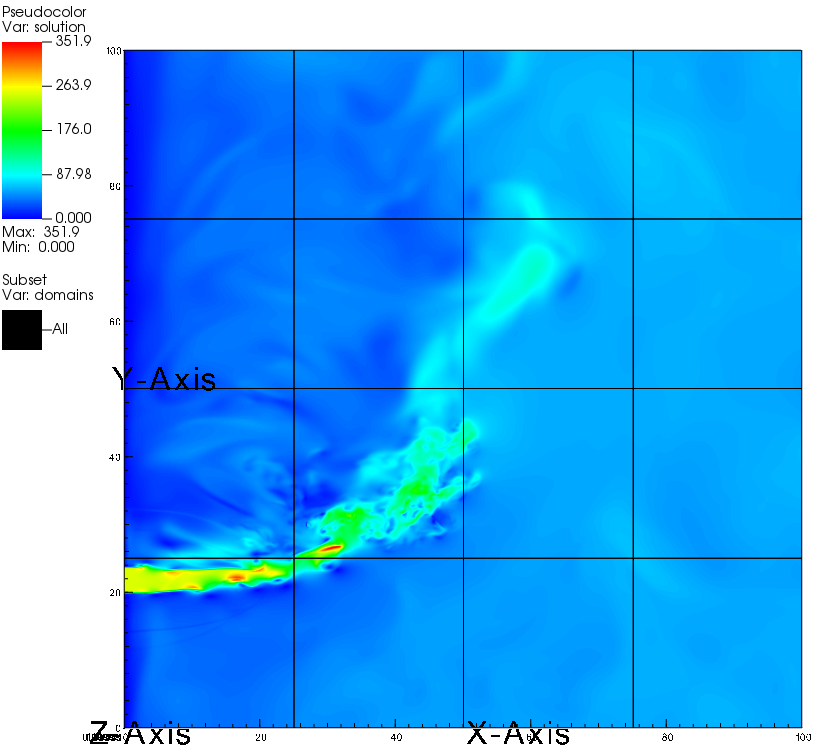
\includegraphics[width=0.45\textwidth]{figures/s3d-2d-profile.png}
	\caption{2-D slice of S3D dataset}
	\label{fig:s3d-adaptive-2d}
\end{figure}

\Remark{show error convergence plots for S3D on 16 subdomains with adaptivity}

\subsubsection{Nek5000 dataset}

\Remark{add table of actual compression and error as $n_s$ is changed}

\Remark{Discuss about complications and potential ways to enforce continuity. (a) Use decoded data, (b) Use control point space across interface}


\subsection{Parallel Scalability}\label{sec:parallel-scalability}

The parallel scalability of the implemented RAS iterative solver for ensuring continuity across block boundaries was measured on the 2-D CESM dataset, whose solution profile in a uniform latitude-longitude grid is shown in \fig{fig:cesm-2d-profile}. 
Our experiments were executed on the Bebop cluster at
Argonne National Laboratory LCRC (Laboratory Computing Resource Center). Bebop has 1024 public nodes, with Intel Broadwell or Intel Knights Landing processors, with 128 GB memory per Broadwell node, and 104 GB per KNL node. It has an Omni-Path Fabric Interconnect. Broadwell processors have 36 cores, while KNL processors have 64 cores. We primarily used the KNL processors for the scalability tests presented below.

A strong scalability test was performed on the Bebop cluster with the climate dataset, using 32 subdomains in X-direction and 128 subdomains in Y-direction. With this fixed DD and 100 control point per subdomain resolution, the driver utilized DIY to handle the block assignment to processes. As the total number of processes used in the parallel run was varied from [1,2,$\ldots$4096], we measured the overall time for the initial subdomain solves, and the consequent RAS iteration cycle for $nMaxASM=5$. The time to compute the MFA in parallel is shown for this strong scalability experiement in \fig{fig:cesm-strong-scalability}.

\begin{figure}
	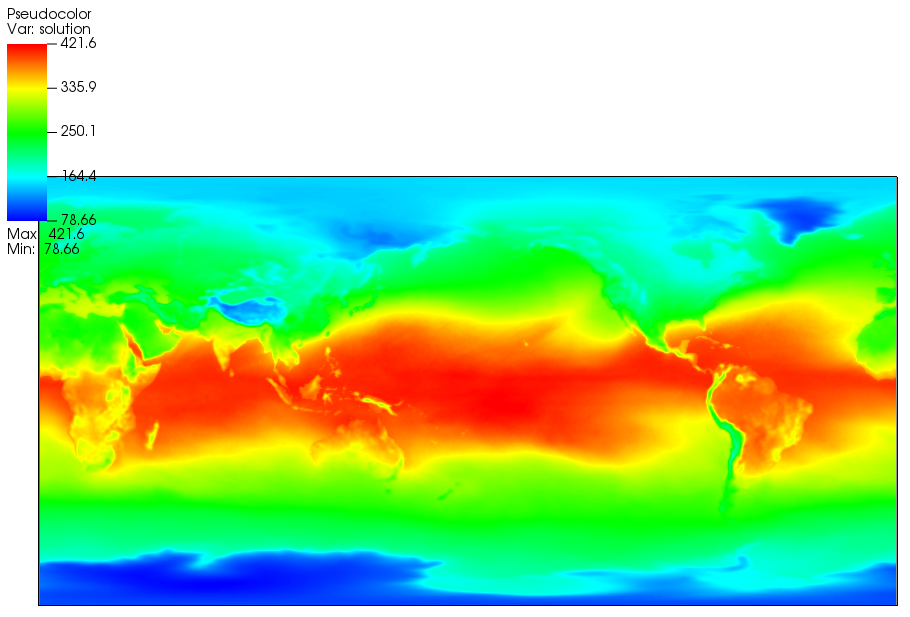
\includegraphics[width=0.45\textwidth]{figures/cesm-profile.png}
	\caption{2-D CESM climate dataset}
	\label{fig:cesm-2d-profile]}
\end{figure}

As expected, the hierarchical iterative scheme with RAS-Krylov combination shows excellent scalability for the chosen dataset and the overall time to compute the MFA was reduced from nearly 7000s on a single process,  to 9.5s on 2048 processes, while ensuring $G_0, G_1$ continuity in the domain interfaces. The ratio of computational work in local subdomain solves in comparison to communication time in nearest-neighbor exchanges gradually increases as subdomain size shrinks. This is due to the fact that global information on smaller subdomains take multiple iterations to propagate, and hence using overlaps for such large problems would be a recommended extension in the future to improve overall scalability of the algorithm.

%CESM dataset has 6.5M data points
%We used 32*128 = 4096 subdomains for the strong scaling test
%\Remark{How does the nearest neighbor communication stay bounded ? measure timings separately ?}

%jobrun_neup cesm_p1 1 1 python ../Projection-2D.py -x 32 -y 128 -p 5 -c 10 -a 5 --disableadaptivity 

\begin{figure}
	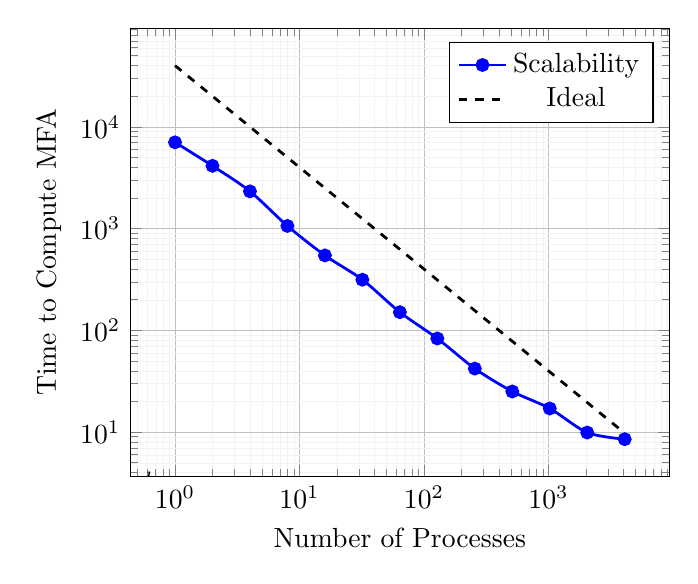
\begin{tikzpicture}
	
	\begin{loglogaxis}[
	legend pos= north east,
%	ymin = 0.0005, ymax = 0.01,
	xlabel=Number of Processes,
	ylabel=Time to Compute MFA,
%	nodes near coords*={\Label},
%	visualization depends on={value \thisrow{label} \as \Label},
	grid=both,
	grid style={line width=.1pt, draw=gray!10},
	major grid style={line width=.2pt,draw=gray!50},
	axis line style={latex-latex},
	every axis plot/.append style={line width=1.0pt},
	%axis lines=middle,
	]
	\axispath\draw
	(7.49165,-10.02171)
	|-  (8.31801,-11.32467)
	node[near start,left] {$\frac{dy}{dx} = -2.58$};
	
	\addplot[smooth,mark=*,blue,width=5pt] table [meta=eff]  {
		x y eff
		1	7045.451504	100
		2	4137.296798	85.14558959
		4	2322.884537	75.82653583
		8	1061.974002	82.92871918
		16	544.925238	80.80754722
		32	314.578249	69.98906001
		64	150.8316872	72.98544611
		128	83.16858159	66.18195096
		256	42.09792775	65.37446476
		512	25.07828297	54.870772
		1024	17.07229925	40.30109616
		2048	9.898160849	34.75556641
		4096	8.519652482	20.18956686
	};

	\addplot[dashed,black,width=2pt] table [meta=class]  {
	x y class 
	1	40000	100
	2	20000	100
	4	10000	100
	8	5000	100
	16	2500	100
	32	1250	100
	64	625	100
	128	312.5	100
	256	156.25	100
	512	78.125	100
	1024	39.0625	100
	2048	19.53125	100
	4096	9.765625	100
};
	
	\legend{Scalability\\Ideal\\}
	
	\end{loglogaxis}
	\end{tikzpicture}
	\caption{Strong Scalability of the 2-D CESM Problem with 4096 subdomains and 100 control points/subdomain}
	\label{fig:cesm-strong-scalability}
\end{figure}


%\paragraph{Positioning Figures and Tables} Place figures and tables at the top and 
%``Fig.~\ref{fig}'', even at the beginning of a sentence.

%\begin{table}[htbp]
%\caption{Table Type Styles}
%\begin{center}
%\begin{tabular}{|c|c|c|c|}
%\hline
%\textbf{Table}&\multicolumn{3}{|c|}{\textbf{Table Column Head}} \\
%\cline{2-4} 
%\textbf{Head} & \textbf{\textit{Table column subhead}}& \textbf{\textit{Subhead}}& \textbf{\textit{Subhead}} \\
%\hline
%copy& More table copy$^{\mathrm{a}}$& &  \\
%\hline
%\multicolumn{4}{l}{$^{\mathrm{a}}$Sample of a Table footnote.}
%\end{tabular}
%\label{tab1}
%\end{center}
%\end{table}

%\begin{figure}[htbp]
%\centerline{\includegraphics{fig1.png}}
%\caption{Example of a figure caption.}
%\label{fig}
%\end{figure}


\section{Conclusion}

We have presented a scalable DD approach to tackle the issue of discontinuous MFA representations when performing the computations in parallel. Jacobi-Schwarz is a natural algorithmic fit for data analysis problems to create performant MFA encoders in parallel. Through the user of Schwarz-based iterative schemes, combined with L-BFGS or Krylov solvers for local subdomain solves, the hierarchic iterative technique was proven to be robust in converging to the compressed functional representation of the given data, without sacrificing the approximation accuracy. Combining NURBS-based adaptivity with a-posteriori error measures, and ensuring higher-order continuity across block boundaries, a scalable infrastructure has been presented. The PyDIY based Python implementations for 1-D and 2-D problems have been shown here to resolve complex solution profiles and gradient variations, even under decreasing subdomain sizes. The use of overlap layers can definitely improve the overall MFA accuracy and convergence speed of the JS algorithm as shown for the 1-D analytical problems, but at a slightly higher cost per iteration. The strong scalability of the algorithm was also explored for a reasonably large 2-D climate dataset {\color{red} talk about 2-d scalability when we have the results}

A more natural way to ensure continuity across NURBS patches would be to use T-splines \cite{sederberg-2004}, which is specifically designed for merging higher-dimensional surfaces with non-matching knot locations. The implementation of T-splines for adaptivity in the context of MFA is currently being explored, and the presented ASM based solver approach can still be used to impose constraints across subdomain patch boundaries, while local constraints within each block to satisfy hanging node DoFs can be imposed with appropriate T-spline basis modifications.

{\color{red} 
	should we talk about implementation of the code in C++ as future work?
	it would also be interesting to use multilevel techniques to create a hierarchical MFA representation and use ASM to accelerate finer solves using coarser control point data. Need to explore this idea further but can propose it here as future exploration topic
}

%\begin{itemize}
%	\item What did we implement to enhance speedup of the MFA framework and did we preserve accuracy of the underlying method ?
%	\item Did we speedup the actual computation by performing DD with ASM global iterations for some of the problem data ?
%	\item Does the method scale as a function of domains and problem size ? 
%	\item What advantages does it provide for fix-up schemes that can be used in a post-processing step (ref Iulian's blending idea) ?
%	\item Future extensions to T-splines and local adaptivity and potential complications involved
%\end{itemize}

\section*{Acknowledgment}

This work is supported by Advanced Scientific Computing Research, Office of Science, U.S. Department of Energy, under
Contract DE-AC02-06CH11357, program manager Laura Biven. We gratefully acknowledge the computing resources provided on
Bebop, a high-performance computing cluster operated by the Laboratory Computing Resource Center (LCRC) at Argonne
National Laboratory.

\bibliographystyle{IEEEtran}
\bibliography{asm-mfa}

%\vspace{12pt}
%\color{red}
%IEEE conference templates contain guidance text for composing and formatting conference papers. Please ensure that all template text is removed from your conference paper prior to submission to the conference. Failure to remove the template text from your paper may result in your paper not being published.

\end{document}
